\documentclass[10pt,a4paper]{article}

% Packages
\usepackage[utf8]{inputenc}
\usepackage[T1]{fontenc}

\usepackage{setspace}          % Pour gérer l'interligne
\usepackage{times}             % Police similaire à Elsevier (Times)
\usepackage{geometry}          % Marges
\usepackage{graphicx}
\usepackage{amsmath}
\usepackage{titlesec}          % Pour régler l'espacement des titres
\usepackage{microtype}         % Améliore la typographie
\usepackage[style=chem-acs,sorting=none]{biblatex}
\usepackage{lipsum}
\usepackage{caption}           % For customizing captions
\usepackage{float}            % For placing figures and tables
\usepackage{siunitx}          % For SI units
\usepackage{subcaption}        % For subfigures

\usepackage[style=chem-acs,sorting=none]{biblatex}

% Geometry settings
\geometry{margin=2.5cm}
\onehalfspacing

% Redefine captions for figures and tables
\captionsetup[figure]{
    labelfont={bf}, % Bold label (e.g., Fig.)
    textfont=it,    % Italic caption text
    labelsep=period, % Separator between label and text
    name={Fig.}     % Prefix for figures
}

\captionsetup[table]{
    labelfont={bf}, % Bold label (e.g., Table.)
    textfont=it,    % Italic caption text
    labelsep=period, % Separator between label and text
    name={Table.}   % Prefix for tables
}

% Redefine command
\renewcommand{\thesection}{\Roman{section}}
\renewcommand{\thesubsection}{\thesection.\Alph{subsection}}
\titlespacing{\section}{0pt}{1.5em}{1em}
\titlespacing{\subsection}{0pt}{1.2em}{0.8em}

% Footpage settings
\usepackage{fancyhdr}
\pagestyle{fancy}
\fancyhf{}
\fancyfoot[R]{\thepage}
\renewcommand{\headrulewidth}{0pt}

\addbibresource{references.bib}

\begin{document}
\begin{figure}
  \begin{minipage}[t]{0.45\textwidth}
      
      
\includegraphics[width=\textwidth]{Figures/EPL.png}
     
      \label{fig:EPL}
  \end{minipage}
  \hfill
  \begin{minipage}[t]{0.45\textwidth}
      \raggedleft
       \textbf{LMAPR2231\\ Metallurgical and electrochemical processes}\\
       
  
  \end{minipage}
\end{figure}
\hrulefill

\begin{center}
    \textbf{\LARGE Electrochemical characterisation of water electrolyzier and fuel cell}\\
    \vspace{0.5cm}
    \textit{\small{N.De Troeyer Janssens - 2471200, F.Clinquart - 59602100\footnote{Institute of Mechanics, Materials and Civil Engineering,Louvain School of Engineering. Louvain-la-neuve, Belgium. } }}\\
    \textbf{\small{\today}}
\end{center}


\section{Introduction}

\lipsum[1]
\lipsum[2]
\lipsum[3]
\textbf{Bien définir PEM et electrolyzer et les abrievation.}\\
\section{Materials and Methods}

The experiments were conducted following the procedures outlined in the reference document \textit{LaboPAC 2025}, available on the Moodle website of the course \cite{labopac2025}, which provides a detailed description of the materials, equipment, and methodologies used.
The laboratory session was divided into two lab sessions. The  first lab session focused on the basic characterization of the water electrolyzer and the PEM fuel cell, while the second lab session involved a more in-depth analysis of the electrochemical processes occurring in fuel cells.
Table. \ref{tab:experimental_summary} is a brief summary of the experimental setup and Objective for the first lab session, which was divided into two main parts: the water electrolyzer experiments and the PEM fuel cell experiments.
Four experiments were conducted during the first lab session. In these document, the experiments are referred to as \textit{Exp1}, \textit{Exp2}, \textit{Exp3}, and \textit{Exp4}.
{\color{red} Preciser quel electerolyseur on a eu et quel fuel cell. + Discuter des resisatnce utilisées}

\begin{table}[H]
    \centering
    \caption{Summary of the four main experimental quantities for Lab Session I, grouped by device type. The analysis done in each experiment is also indicated.}
    \renewcommand{\arraystretch}{2} % Adjust row height
    \setlength{\tabcolsep}{6pt} % Adjust column spacing
    \begin{tabular}{|p{2cm}|p{4cm}|p{4cm}|p{4cm}|}
        \hline
        \textbf{Experiment} & \textbf{Objective} & \textbf{Measured Quantities} & \textbf{Analysis} \\
        \hline
        \multicolumn{4}{|c|}{\textbf{A – Water Electrolyzer Experiments}} \\
        \hline
        \textit{Exp1} & Determine the water decomposition voltage & Voltage (\textbf{U}), Current \textbf{(I)} for various resistances & Plot {current} vs. {voltage}, identify gas onset voltage, compare with theoretical value \\
        \hline
        \textit{Exp2} & Evaluate efficiency of hydrogen production & Time \textbf{t}, Applied voltage \textbf{(U)}, Current \textbf{I}, Volume of ${H_2}$ $\mathbf{v_{H_2}} $produced & Plot $H_2$ volume vs. time, calculate energy and Faraday efficiencies \\
        \hline
        \multicolumn{4}{|c|}{\textbf{B – PEM Fuel Cell Experiments}} \\
        \hline
        \textit{Exp3} & Identify maximum power output of the cell & Voltage \textbf{ (V)}, Current \textbf{ (A)} for various resistances & Plot {voltage} vs. {current} and {power} vs. {current}, determine Maximum Power Point (MPP) \\
        \hline
        \textit{Exp4} & Evaluate efficiency during hydrogen consumption & Time \textbf{t}, Voltage \textbf{U}, Current \textbf{I}, Volume of ${H_2}$ $\mathbf{v_{H_2}}$ consumed & Plot ${H_2}$ consumption vs. time, calculate energy and Faraday efficiencies \\
        \hline
    \end{tabular}
    \vspace{0.5em}
    
    \label{tab:experimental_summary} % Added label for referencing
\end{table}


\begin{table}[H]
    \centering
    \begin{minipage}{0.45\textwidth}
        \centering
        \caption{\textit{Exp1: Measured resistance, voltage, and current for the water electrolyzer.}}
        \renewcommand{\arraystretch}{1.4} % Adjust row height
        \setlength{\tabcolsep}{8pt} % Adjust column spacing
        \begin{tabular}{|c|c|c|}
            \hline
            \textbf{R (\si{\ohm})} & \textbf{U (\si{\volt})} & \textbf{I (\si{\ampere})} \\
            \hline
            0 & 0 & 0 \\
            \hline
            0.1 & 0.105 & 0 \\
            \hline
            0.33 & 0.67 & 0 \\
            \hline
            1 & 1.43 & 0 \\
            \hline  
            3.3 & 3.19 & 0.24 \\
            \hline
            10 & 3.52 & 0.8 \\
            \hline
            33 & 3.64 & 1.04 \\
            \hline
            100 & 3.68 & 1.1 \\
            \hline
            330 & 3.69 & 1.14 \\
            \hline
        \end{tabular}
        \label{tab:exp1_results}
    \end{minipage}
    \hfill
    \begin{minipage}{0.45\textwidth}
        \centering
        \caption{\textit{Exp3: Measured resistance, voltage, current, and power for the PEM fuel cell.}}
        \renewcommand{\arraystretch}{1.4} % Adjust row height
        \setlength{\tabcolsep}{8pt} % Adjust column spacing
        \begin{tabular}{|c|c|c|c|}
                    \hline
                    \textbf{R (\si{\ohm})} & \textbf{U (\si{\volt})} & \textbf{I (\si{\ampere})} & \textbf{P (\si{\milli\watt})} \\
                    \hline
                    $\infty$ & 0.898 & 0 & 0.0 \\
                    \hline
                    330 & 0.8 & 0.0025 & 2.0 \\
                    \hline
                    100 & 0.76 & 0.0074 & 5.624 \\
                    \hline
                    33 & 0.71 & 0.0203 & 14.413 \\
                    \hline
                    10 & 0.65 & 0.0512 & 33.28 \\
                    \hline
                    3.3 & 0.61 & 0.0975 & 59.475 \\
                    \hline
                    1 & 0.48 & 0.124 & 59.52 \\
                    \hline
                    0.33 & 0.354 & 0.1092 & 38.6568 \\
                    \hline
                    0.1 & 0.33 & 0.1045 & 34.485 \\
                    \hline
                    0 & 0.325 & 0.1018 & 33.085 \\
                    \hline
                \end{tabular}
                \label{tab:exp3_results}
            \end{minipage}
    \vspace{1cm}
    \begin{minipage}{0.45\textwidth}
        \centering
        \caption{\textit{Exp2: Measured volume, current, and time for the water electrolyzer.}}
        \renewcommand{\arraystretch}{1.4} % Adjust row height
        \setlength{\tabcolsep}{8pt} % Adjust column spacing
        \begin{tabular}{|c|c|c|}
            \hline
            \textbf{$v_{exp}$ (\si{\centi\meter\cubed})} & \textbf{I (\si{\ampere})} & \textbf{t (\si{\second})} \\
            \hline
            0 & 0 & 0 \\
            \hline
            10 & 1 & 18 \\
            \hline
            20 & 0.98 & 60 \\
            \hline
            30 & 0.98 & 98.5 \\
            \hline
            40 & 0.97 & 139.8 \\
            \hline
            50 & 0.97 & 174.6 \\
            \hline
            60 & 0.97 & 227.2 \\
            \hline
            70 & 0.97 & 273.5 \\
            \hline
            80 & 0.97 & 314.5 \\
            \hline
        \end{tabular}
        \label{tab:exp2_results}
    \end{minipage}
    \hfill
    \begin{minipage}{0.45\textwidth}
        \centering
        \caption{\textit{Exp4: Measured time, voltage, current, and hydrogen volume for the PEM fuel cell.}}
        \renewcommand{\arraystretch}{1.4} % Adjust row height
        \setlength{\tabcolsep}{8pt} % Adjust column spacing
        \begin{tabular}{|c|c|c|c|}
            \hline
            \textbf{t (\si{\second})} & \textbf{U (\si{\volt})} & \textbf{I (\si{\ampere})} & \textbf{$v_{exp}$ (\si{\centi\meter\cubed})} \\
            \hline
            0 & 0.35 & 0.055 & 0 \\
            \hline
            490 & 0.413 & 0.0762 & 2.5 \\
            \hline
            639 & 0.484 & 0.078 & 5 \\
            \hline
            918 & 0.492 & 0.0791 & 7.5 \\
            \hline
            1122 & 0.493 & 0.0786 & 10 \\
            \hline
            1380 & 0.49 & 0.0786 & 12.5 \\
            \hline
            1620 & 0.484 & 0.0786 & 15 \\
            \hline
        \end{tabular}
        \label{tab:exp4_results}
    \end{minipage}
\end{table}



\begin{figure}[H]
    \centering
    \begin{subfigure}[t]{0.45\textwidth}
        \centering
        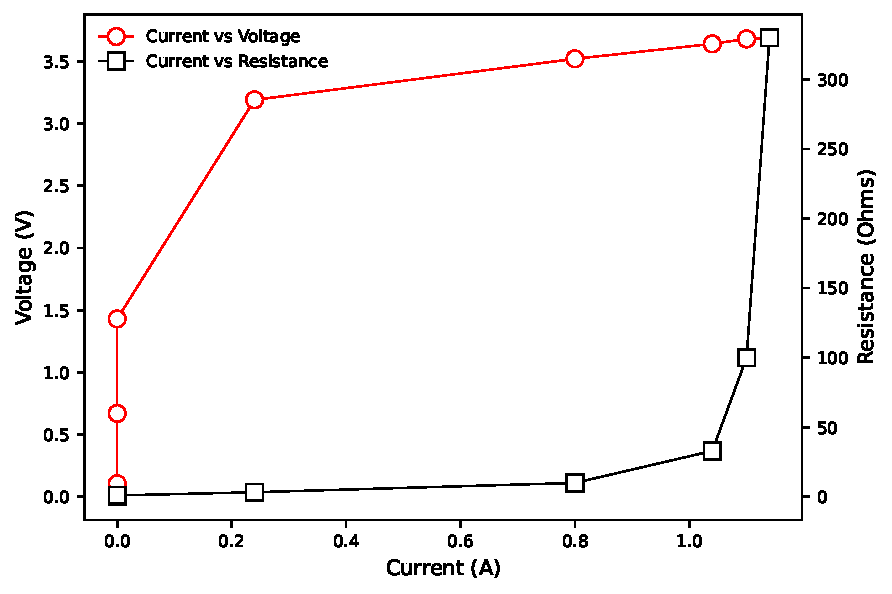
\includegraphics[width=\textwidth]{Output/Exp1.pdf}
        \caption{Voltage vs. Current for Experiment 1.}
        \label{fig:summary_results:exp1}
    \end{subfigure}
    \hfill
    \begin{subfigure}[t]{0.45\textwidth}
        \centering
        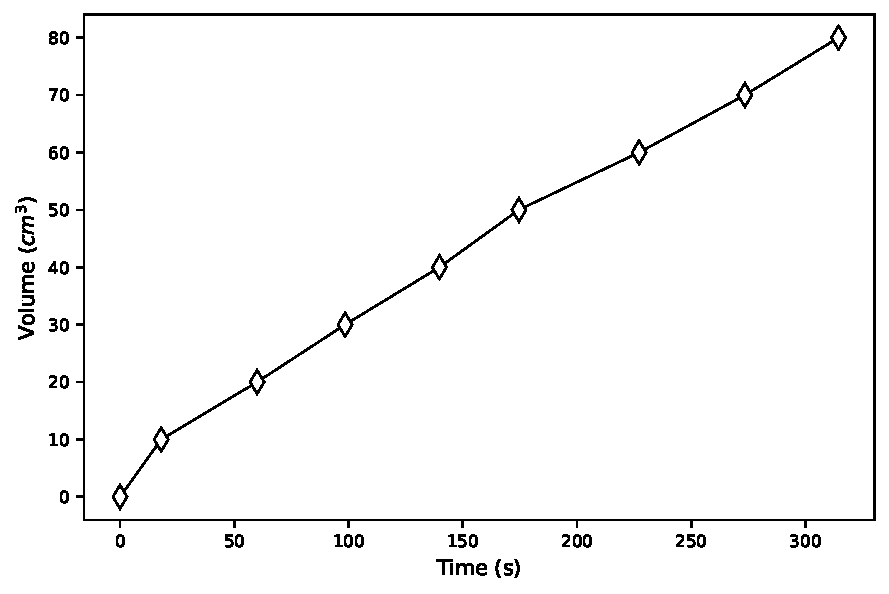
\includegraphics[width=\textwidth]{Output/Exp2.pdf}
        \caption{Time vs. Volume for Experiment 2.}
        \label{fig:summary_results:exp2}
    \end{subfigure}

    \vspace{1cm}  % Optional: Adjust or remove if spacing looks odd

    \begin{subfigure}[t]{0.45\textwidth}
        \centering
        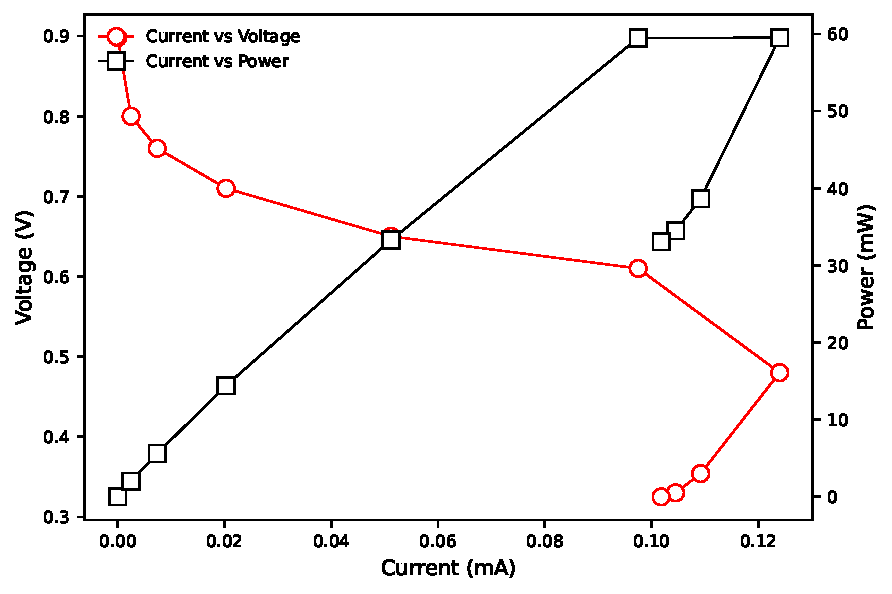
\includegraphics[width=\textwidth]{Output/Exp3_power.pdf}
        \caption{Power vs. Current for Experiment 3.}
        \label{fig:summary_results:exp3}
    \end{subfigure}
    \hfill
    \begin{subfigure}[t]{0.45\textwidth}
        \centering
        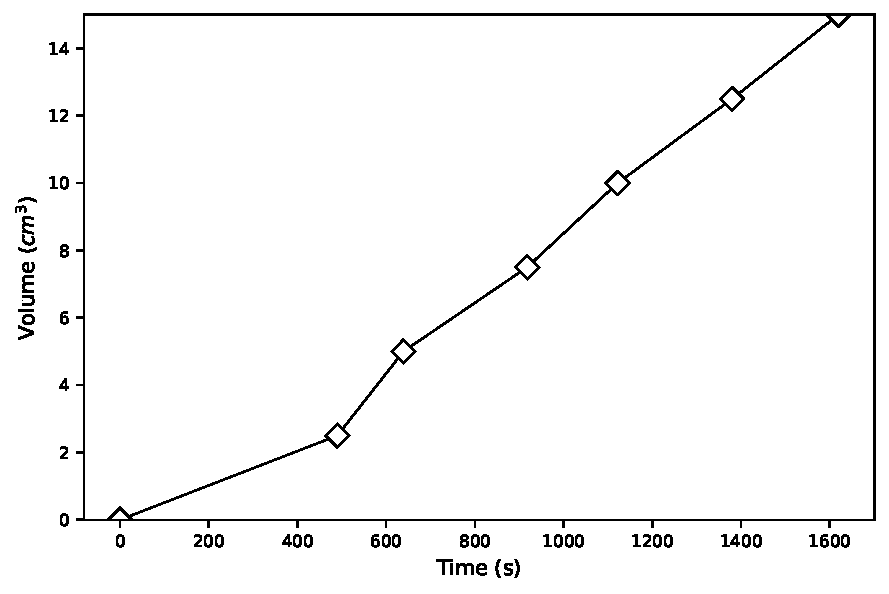
\includegraphics[width=\textwidth]{Output/Exp4.pdf}
        \caption{Time vs. Volume for Experiment 4.}
        \label{fig:summary_results:exp4}
    \end{subfigure}

    \caption{Summary of experimental results for the water electrolyzer and PEM fuel cell.}
    \label{fig:summary_results}
\end{figure}

\section{Discussion}
\subsection{Theoretical Background}

The reaction in a PEM fuel cell is given in Table \ref{tab:PEM_fuel_cell_reactions}.
\begin{table}[H]
\centering
\caption{Reactions at the electrodes and overall reaction for a PEM fuel cell.}
\begin{tabular}{|c|c|c|}
\hline
\textbf{Electrode} & \textbf{Reaction} & \textbf{Location} \\ \hline
Anode & $H_{2(g)} \xrightarrow{} 2H^+_{(aq)} + 2e^-$ & Oxidation \\ \hline
Cathode & $O_{2(g)} + 4e^- + 4H^+_{(aq)} \xrightarrow{} 2H_2O_{(l)}$ & Reduction \\ \hline
Overall Reaction & $O_{2(g)} + 2H_{2(g)} \xrightarrow{} 2H_2O_{(l)}$ & - \\ \hline
\end{tabular}
\label{tab:PEM_fuel_cell_reactions}
\end{table}

The Nernst equation gives the cell potential:
\begin{equation}
    V_{eq} = V^{\circ}_{eq} - \frac{RT}{zF} \ln \left( \frac{a_{red}}{a_{ox}} \right) = V^{\circ}_{eq} - \frac{RT}{zF} \ln \left( \frac{a_{H_2O}}{a_{H_2}^2 a_{O_2}} \right)
\end{equation}

\begin{minipage}{0.6\textwidth}
where $V^{\circ}_{eq}$ is the standard cell potential, $R$ is the gas constant, $T$ is the temperature in Kelvin, $n$ is the number of electrons involved in the reaction, $F$ is the Faraday constant, and $a_{H_2O}$, $a_{H_2}$, and $a_{O_2}$ are the activities of the species involved in the reaction. Since water is liquid, the activity of water is assumed to be 1. The activities of the gases are assumed to be equal to their partial pressures divided by the standard pressure (1 bar). Moreover, the pressure of the oxygen is assumed to be equal to the pressure of the hydrogen and is equal to $P$, the service pressure of the electrolyzer (1 bar) \cite{SocChimFr1995}. Notice that the oxydation and reduction reaction at the electrode is function of the concentration of hydrogen ions in the electrolytes,i.e. the pH. The equilibrium potential can be computed thanks to the Nernst equation, this computation is made in the \textit{LMAPR2231 Metallurgical and Electrochimical Course} \cite{uclouvain_lmapr2231}. 
The E-pH diagram is shown at the Figure \ref{fig:PEM_fuel_cell}. It is important to note that the reaction at the electrode and at the cathode have the same slope. In induce that, since the cell potential is the difference of the equilibrium potential at the anode and at the cathode, the cell potential is indepedent of the pH.
\end{minipage}
\hfill
\begin{minipage}{0.35\textwidth}
\begin{figure}[H]
    \centering
    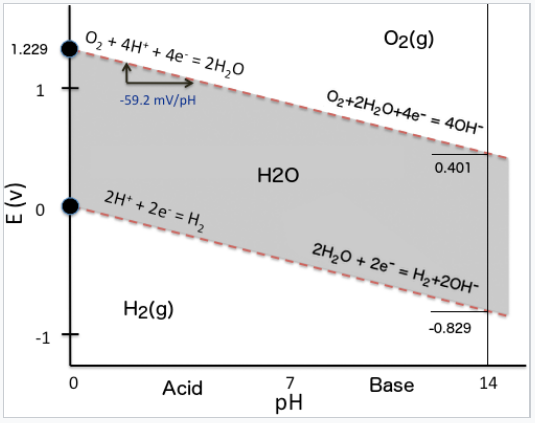
\includegraphics[width=\textwidth]{Figures/Pourbaix_water.png}
    \caption{E-pH diagram of water. The diagram shows the thermodynamic stability of water in terms of its potential (E) and pH. The shaded area indicates the region where water is stable, while the lines represent the boundaries between different species \cite{LibreTextsElectrochemicalPotentials}.}
    \label{fig:PEM_fuel_cell}
    -
\end{figure}
\end{minipage}

At the standard conditions, we can determine the Gibbs free energy change of the overall electrochemical reaction from the cell potential at those conditions thanks to this formula: 
\begin{equation}
    -\Delta G^{\circ} = n \cdot F \cdot V^{\circ}_{eq}
\end{equation} 
where $V^{\circ}_{cell,eq} = V^{\circ}_{cathode} - V^{\circ}_{anode}$, n is the number of electrons involved in the reaction, 4 in this case, and F is the Faraday constant. 
From the Table \ref{tab:cell_potentials}, The standard electrode potentials are $V^{\circ}_{anode} = 0$ and $V^{\circ}_{cathode} = 1.229$. The cell potential is $V^{\circ}_{cell,eq} = 1.229$. This is the maximun value of potential that can be deliver by the fuel cell, when no current is taken. The standard Gibss free energy is $G^{\circ} = - 474.32 \frac{kJ}{2 mol(H_2O)} = -237.16 \frac{kJ}{mol} = -56.64 \frac{kcal}{mol}$. This is consistent with the Gibbs free energy change of the overall electrochemical reaction of Hydrogen shonw in the Table. \ref{tab:cell_potentials}. 
\begin{table}[H]
\centering
\caption{Theoretical Cell Potentials of Various Oxidation Reactions at 25°C.}
\begin{tabular}{|c|c|c|c|}
\hline
\textbf{Fuel} & \textbf{Reaction} & $\mathbf{\Delta G^0}$ (kcal mol$^{-1}$) & $\mathbf{V_a^0}$ (V) \\ \hline
Hydrogen & $H_2 + \frac{1}{2}O_2 \rightarrow H_2O$ & -56.69 & 1.229 \\ \hline
         & $H_2 + Cl_2 \rightarrow 2HCl$ & -62.70 & 1.370 \\ \hline
Propane  & $C_3H_8 + 5O_2 \rightarrow 3CO_2 + 4H_2O$ & -503.90 & 1.093 \\ \hline
Methane  & $CH_4 + 2O_2 \rightarrow CO_2 + 2H_2O$ & -195.50 & 1.060 \\ \hline
Carbon monoxide & $CO + \frac{1}{2}O_2 \rightarrow CO_2$ & -61.45 & 1.333 \\ \hline
Ammonia  & $NH_3 + \frac{3}{2}O_2 \rightarrow \frac{3}{2}H_2O + \frac{1}{2}N_2$ & -80.8 & 1.170 \\ \hline
Methanol & $CH_3OH + \frac{3}{2}O_2 \rightarrow CO_2 + 2H_2O$ & -168.95 & 1.222 \\ \hline
Formaldehyde & $CH_2O + O_2 \rightarrow CO_2 + H_2O$ & -124.7 & 1.350 \\ \hline
Formic acid & $HCOOH + \frac{1}{2}O_2 \rightarrow CO_2 + H_2O$ & -68.2 & 1.480 \\ \hline
Hydrazine & $N_2H_4 + O_2 \rightarrow N_2 + 2H_2O$ & -143.9 & 1.560 \\ \hline
Zinc      & $Zn + \frac{1}{2}O_2 \rightarrow ZnO$ & -76.05 & 1.650 \\ \hline
Sodium    & $Na + \frac{1}{2}H_2O + \frac{1}{2}O_2 \rightarrow NaOH$ & -71.84 & 3.120 \\ \hline
Carbon    & $C + O_2 \rightarrow CO_2$ & -94.26 & 1.020 \\ \hline
\end{tabular}
\label{tab:cell_potentials}
\end{table}
  

The same reasoning can be done for a PEM electrolyzer producing oxygen and hydrogen. The reactions at the electrodes in this case would be:
\begin{table}[H]
\centering
\caption{Reactions at the electrodes and overall reaction for a PEM electrolyzer.}
\begin{tabular}{|c|c|c|}
\hline
\textbf{Electrode} & \textbf{Reaction} & \textbf{Location} \\ \hline
Anode & $2H_{2}O_{(l)} \xrightarrow{} O_{2(g)} + 4e^- + 4H^+_{(aq)}$ & Oxidation \\ \hline
Cathode & $4H^+_{(aq)} + 4e^- \xrightarrow{} 2H_{2(g)}$ & Reduction \\ \hline
Overall Reaction & $O_{2(g)} + 2H_{2(g)} \xrightarrow{} 2H_2O_{(l)}$ & - \\ \hline
\end{tabular}
\label{tab:PEM_electrolyzer_reactions}
\end{table}
A PEM electrolyzer works like a PEM fuel cell but in reverse.  However, the key difference is that in an electrolyzer, this voltage represents the minimum required to start the reaction, rather than the maximum produced.
The standard electrode potential at the anode and the cathode are respectively $V^{\circ}_{anode} = 1.229$ and $V^{\circ}_{cathode} = 0$ which gives a negative standard cell potential $V^{\circ}_{cell,eq} = -1.229$ and thus a positive Gibbs free energy at the standard condition $G^{\circ} = 474.32 \frac{kJ}{2 mol(H_2O)} = 237.16 \frac{kJ}{mol} = 56.64 \frac{kcal}{mol}$. 
This global reaction is thus not thermodynamically favored at the standard conditions \cite{wikiWaterElectrolysisThermo}.
\subsection{Faradic Efficiency}

The theoretical volume of hydrogen produced, $v_{theo}$, is given by:
\begin{equation}
    v_{theo} = \frac{i \cdot t \cdot R \cdot T}{z \cdot F \cdot p}
\end{equation}
where $i$ is the current, $t$ is the time, $R$ is the gas constant, $T$ is the temperature, $z$ is the number of electrons involved in the reaction ($z = 2$ for hydrogen), $F$ is the Faraday constant, and $p$ is the pressure.

The Faradic efficiency, $\eta_{Farad}$, is calculated as:
\begin{equation}
    \eta_{Farad} = \frac{v_{exp}}{v_{theo}} \times 100
\end{equation}

\begin{table}[H]
    \centering
    \caption{Faradic efficiencies of each measurement for Experiment 4.}
    \begin{tabular}{|c|c|c|c|c|}
        \hline
        $v_{exp}$ (\si{\centi\meter\cubed}) & $i$ (\si{\ampere}) & $t$ (\si{\second}) & $v_{theo}$ (\si{\centi\meter\cubed}) & $\eta_{Farad}$ (\%) \\
        \hline
        0 & - & - & - & - \\
        \hline
        2.5 & 0.0762 & 490 & 2.8 & 89.3 \\
        \hline
        5 & 0.078 & 639 & 5.2 & 96.2 \\
        \hline
        7.5 & 0.0791 & 918 & 7.8 & 96.1 \\
        \hline
        10 & 0.0786 & 1122 & 10.1 & 99.0 \\
        \hline
        12.5 & 0.0786 & 1380 & 12.4 & 100.8 \\
        \hline
        15 & 0.0786 & 1620 & 14.8 & 101.4 \\
        \hline
    \end{tabular}
    \label{tab:eta_farad_exp4}
\end{table}

\subsection{Experimental Results}
\subsubsection{Exp1: Water Decomposition Voltage}


Figure. \ref{fig:summary_results:exp1} shows the voltage as a function of the current and the current as a function of the resistance. The voltage increase rapidly with the current before reaching a plateau. There is no current until the voltage reach 3.19 $\si{V}$. This value is a lot above the theoretical value of 1.23 $\si{V}$. 
The change of slope means that the reaction is starting. Gas bubbles are formed on the electrodes. The different between the theoretical and experimental value may be due to the fact to lost in the electrical circuit and by the fact that only discrete values of resistance was tested. {\color{red} note du degagement gazeux}

\subsubsection{Exp2: Efficiency of Hydrogen Production}
From the experiment 1, the power consumed by the electrolyzer is given by the product of the current and the voltage. Taking the data from The Table \ref{tab:exp1_results}, the power can be computed and plotted as a function of the resistance. 
\begin{figure}[H]
    \centering
    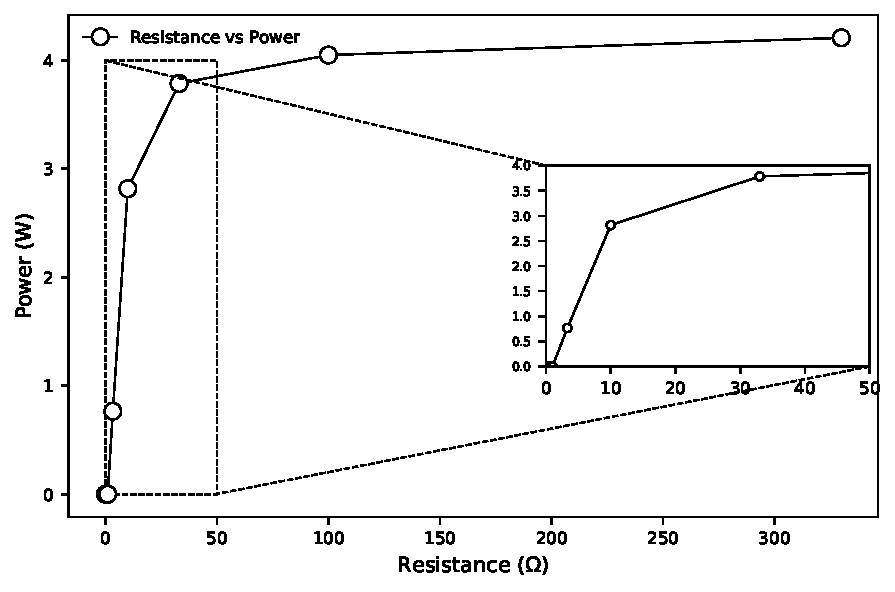
\includegraphics[width=0.7\textwidth]{Output/Exp1_R_vs_power_with_zoom.pdf}
    \caption{Power as a function of the resistance for Exp1. The zoom on the right shows the power for resistances between 0 and 50 $\si{\ohm}$.}
    \label{fig:summary_results:exp1}
\end{figure}
For this experiment, a resistance of 33$\Omega$ was chosen. From experiment 1, it was observed that higher resistance leads to higher power. However, since the volume of gas is proportional to the current (see Eq. \ref{eq: v_theo}), a trade-off was made between efficiency and data accuracy. A resistance of 33$\Omega$ was deemed a good compromise.

The average production rate was calculated by taking the mean of $\frac{\Delta v}{\Delta t}$ between each successive data point. This resulted in an average production rate of 0.276 cm$^3$/s.

Assuming the produced hydrogen is dry and behaves as an ideal gas, the theoretical volume can be calculated using the equation:
\begin{equation}
    v_{theo} = \frac{i \cdot t \cdot R \cdot T}{z \cdot F \cdot p} \label{eq: v_theo}
\end{equation}
where $T$ is the ambient temperature, $p$ is the atmospheric pressure, and $n$ is the number of moles. The number of moles $n$ is related to the time $t$ and current $i$ by Faraday’s law of electrolysis: $i \cdot t = n \cdot z \cdot F$, where $z$ is the number of electrons involved in the reaction, which is 4 in this case. The relation between the volume and the number of moles is given by the ideal gas law: $pv = nRT$.
The table below gives the $v_{exp}$, $v_{theo}$ and $\eta_{Farad}$ associated to the time and current points taken during the experiment as 
\begin{equation}
    \eta_{Farad} = \frac{v_{exp}}{v_{theo}}
\end{equation}

\begin{figure}[H]
    \centering
    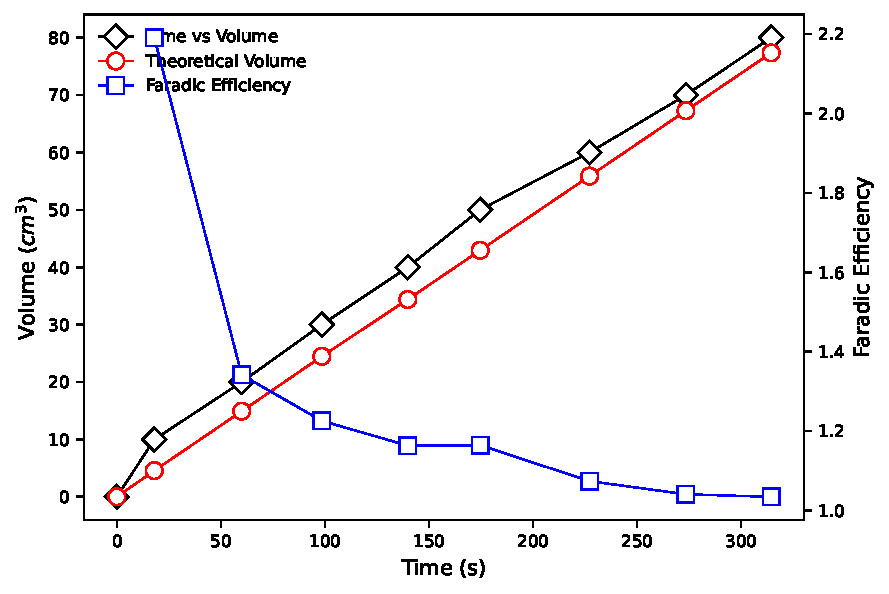
\includegraphics[width=0.7\textwidth]{Output/Exp2_vs_theo.pdf}
    \caption{Volume of hydrogen produced as a function of time for Exp2 with the theoretical volume. The red line is the theoretical volume of hydrogen produced. The blue line is the Faradic efficiency. }
    \label{fig:summary_results:exp2}
\end{figure}

\begin{table}[H]
    \centering
    \caption{Faradic efficiencies of each measurement for Experiment 2.}
    \begin{tabular}{|c|c|}
        \hline
        $v_{exp}$ (\si{\centi\meter\cubed}) & $\eta_{Farad}$ (\%) \\
        \hline
        0 & - \\
        10 & 89.1 \\
        20 & 54.6 \\
        30 & 49.9 \\
        40 & 47.3 \\
        50 & 47.4 \\
        60 & 43.7 \\
        70 & 42.3 \\
        80 & 42.1 \\
        \hline
    \end{tabular}
    \label{tab:eta_farad_exp2}
\end{table}
{\color{red} Discutter + Je n'arrive pas à avoir le même rendement faradique que toi}

\subsubsection{Exp3: Maximum Power Output of the Cell}
The Maximun power point (MPP) is the value of current density and voltage that maxime the power. The resistance that gives the MPP is $1$ $\Omega$ with a power of $59.5$ $\si{mW}$. 

\subsubsection{Exp4: Efficiency during Hydrogen Consumption}

For this experiment, we chose a resistance of 1$\Omega$. This seemed to be the best choice since, from experiment 3, we calculated that it was the resistance that gives the most power.

Following the same reasoning as for experiment 2, we found the Faradic efficiency for each measurements in Table \ref{tab:eta_farad_exp4}.

\section{Conclusion}
\lipsum[5]

\printbibliography




\end{document}
